\documentclass[12pt, a4paper, titlepage]{report}
\usepackage{polski}
\usepackage[utf8]{inputenc}
\usepackage[T1]{fontenc}
\usepackage{indentfirst}
\usepackage{geometry}
\newgeometry{tmargin=2.5cm, bmargin=2.5cm, lmargin=3.5cm, rmargin=2.5cm}
\setlength{\parindent}{0.8cm}
\linespread{1.3}
\usepackage{times}
\usepackage{bchart}
\usepackage{underscore}
\usepackage{xcolor}
\usepackage{array}
\usepackage{pgf-pie}
\usepackage{pgfplots}
\pgfplotsset{width=12cm,compat=newest}
\interfootnotelinepenalty=10000
\raggedbottom

%opening
\author{Dominika Cygankiewicz}
\title{\textbf{Wizerunek subkultury heavymetalowej w~Polsce}}
\date{}

\begin{document}
	
\maketitle
\tableofcontents
\thispagestyle {empty}
%\setlength{\parskip}{1ex plus 0.5ex minus 0.2ex}
\newpage

\chapter*{Wstęp}
\addcontentsline{toc}{chapter}{Wstęp}

\chapter{Subkultura heavymetalowa}
\section{Czym jest subkultura?}
Termin "subkultura" po raz pierwszy pojawił się w~latach 80. XIX wieku w~dziedzinie biologii, gdzie służył do opisywania kultur mikroorganizmów.\footnote{W. Wrzesień, \textit{Krótka historia młodzieżowej subkulturowości}, Warszawa 2013, PWN, s. 40.} W obszarze nauk społecznych zaczął funkcjonować dopiero w~latach 40. XX wieku, za sprawą Miltona M. Gordona, który w~artykule \textit{The Concept of the Sub-Cultur and Its Application.} pisał o subkulturze jako "pododdziale kultury narodowej". \footnote{M. Gordon, \textit{The Concept of the Sub-Cultur and Its Application}, [w:] \textit{Social Forces}, Volume 26, Issue 1, 1947, s. 40–42.} M. M. Gordon, konieczność wprowadzenia pojęcia "subkultura" upatrywał w~braku istniejącego terminu charakteryzującego pomniejsze kultury, wykształcające się w~określonych grupach społecznych: ekonomicznych, regionalnych, etnicznych i~religijnych. W jego rozumieniu, tak uformowane subkultury, miały znaczący wpływ na, przynależące do nich i uczestniczące w~nich, poszczególne jednostki.\footnote{Tamże.} %sprawdzić

% podejmowano różnych prób zdefiniowania zjawiska. Napotkane przez badaczy, trudności definicyjne mogły świadczyć o złożoności i~wielowątkowości prezentowanego problemu.
%Mówiąc o rozwoju zainteresowania socjologów przedmiotem subkulturowości, Witold Wrzesień wyróżnia 3 okresy studiów subkulturowych.

Sformułowana przez M. M. Gordona teza pozwoliła na "uelastycznienie pojęcia subkultury"\footnote{W. Wrzesień, op. cit., s. 41.} i stanowiła pierwszy przystanek na drodze do wyjaśnienia zjawiska. W kolejnych latach studiów subkulturowych, dążono do wypracowania możliwie jak najbardziej kompleksowej definicji, ale wielość prac badawczych oznaczała wiele różnorodnych punktów widzenia i~prób ujęcia badanego problemu. 

M. M. Gordon w swoich rozważaniach unikał powiązania grup subkulturowych z działalnością dewiacyjną, jednak przez długi czas, subkultury były kojarzone z odstępstwami od przyjętych norm kulturowych i~rewoltą.\footnote{M. Pęczak, \textit{Mały słownik subkultur młodzieżowych}, Warszawa 1992, Semper, s. 3.} Pierwotnie, socjologowie zwykli określać mianem subkulturowości grupy nieprzystosowane społecznie i spatologizowane. W roku 1955 Albert Cohen, ich istnienie argumentował poszukiwaniem wśród zbiorowości składającej się z indywidualnych jednostek, rozwiązania problemów wynikających z prób adaptacji.\footnote{A. K. Cohen, \textit{Deliquent Boys, The Culture of the Gang,} 1995, New York: The Free Press, s. 148.} Choć na przestrzeni lat badań socjologicznych, obok jego teorii wykształciło się wiele kontrastowych twierdzeń, w rozumieniu potocznym, subkultury wciąż przywodzić mogą na myśl patologie i~dewiacje.\footnote{M. Filipiak, \textit{Od subkultury do kultury alternatywnej,} Lublin 2003, Wydawnictwo UMCS, s. 13} Obecnie, w~przynależności młodych ludzi do subkultur często upatruje się przyczyny przestępczości wśród nieletnich. Dla służb porządkowych wprowadzane są specjalne podręczniki traktujące o polskich subkulturach, w~skrócie charakteryzujące subkultury występujące w~Polsce i~przyczyny ich powstawania. Wśród nich wymienia się między innymi brak perspektyw samorealizacji, zaburzenia rodzinnych więzi emocjonalnych oraz destrukcyjne formy zachowań propagowane przez media.\footnote{M. Śmiałek, \textit{Subkultury młodzieżowe w~Polsce. Wybrane zagadnienia,} Legionowo 2015, Wydział Wydawnictw i~Poligrafii, s. 12.} Z raportów policyjnych oraz podobnych podręczników, wynikałoby zatem, że przynależność do grup subkulturowych wiąże się z niewłaściwym przebiegiem procesu socjalizacji. Taka kategoryzacja, stawia członków subkultur w~mało przychylnym świetle. 

Etymologia słowa również wskazuje pewne negatywne wzorce interpretacyjne pojęcia i przyczynia się do takiegoż rozumienia jego sensu. Słowo "subkultura" jest odpowiednikiem angielskiego terminu \textit{subculture}, który w~tłumaczeniu na język polski, oznacza tyle, co \textit{podkultura}. Określenie to, w~języku polskim budzi konotacje nacechowane pejoratywne.\footnote{M. Pęczak, op. cit., s. 3.} Silniej zaznacza istnienie kulturowej hierarchii, w~której to podkultura plasuje się pod kulturą \textit{nadrzędną}. Termin "subkultura" posiada mniej deprecjonujący charakter i~jest emocjonalnie neutralny, choć przedrostek "sub-" bezsprzecznie sugeruje pochodność subkultury od kultury. By uniknąć wartościowania, obowiązującym określeniem w języku polskim pozostaje "subkultura". Jak podaje Marian Filipak, obejmuje ono swoim zakresem, pojawiające się w rozprawach naukowych przy temacie subkulturowości, pojęcia "kontrkultury" i "kultury alternatywnej".\footnote{M. Filipak, op. cit., s. 16.}

Termin kontrkultura pojawił się pod koniec lat 60. XX wieku, wraz z początkiem zjawiska kontestacji, i oznaczał sprzeciw wobec zastanej kultury.\footnote{Tamże, s. 14.} Z czasem, kontrkultura zaczęła także wytwarzać w jej miejsce nowe wzorce kulturowe -- formowała kulturę alternatywną. Przez część socjologów, subkultura uznawana jest za fazę wstępną procesu, którego rezultat stanowi kultura alternatywna.\footnote{M. Pęczak, op. cit., s. 4.}

%Analiza naukowa winna być jednak pozbawiona czynników wartościujących. 
%W próbie zdefiniowania zjawiska subkulturowości nie jest to jednak wyznacznik wystarczający. 
Mirosław Pęczak definiuje subkulturę jako spójną grupę społeczną, wyrażającą swoją odmienność poprzez negację utrwalonych wzorów kultury i pozostającą na marginesie dominujących tendencji życia społecznego.\footnote{Tamże, s. 4.} Podobną tezę stawia M. Filipak, który nacisk w swej teorii kładzie na chęć ulepszenia kultury zastanej.\footnote{M. Filipak, op. cit., s. 17.} Socjolog zaznacza, że celem subkulturowości nie jest obalenie dominujących wzorców kulturowych. Nie oznacza to jednak, że owe wzorce są przez nią respektowane. Grupy subkulturowe nie mogą powstawać w próżni społecznej -- muszą istnieć w opozycji do kultury, z której się wywodzą.\footnote{T. Paleczny, \textit{Grupy subkultury młodzieżowej. Próba analizy -- propozycje teoretyczne,} "Kultura i społeczeństwo", t. 37, nr 3, 1993, s. 179-190.} Jeśli przyjmuje się, że potrzeba uczestnictwa w subkulturze, wywodzi się z buntu, musi istnieć zespół norm, wobec którego owa subkultura może się buntować. W ujęciu R. Dyoniziaka, pomija się jednak aspekt rewolty. W tym rozumieniu, subkultura jest niczym innym, jak zbiorem wartości, norm i wzorów, wytworzonych przez wiele jednostek mających podobne problemy i wspólne zainteresowania i dążenia, połączonych trwałą więzią.\footnote{R. Dyoniziak, \textit{Młodzieżowa podkultura,} Warszawa 1965, Wiedza Powszechna, s. 11.} 

Słowa "subkultura" używano zatem do określania zarówno grup przestępczych, etnicznych, zawodowych, religijnych, ekonomicznych, jak i ruchów społecznych. Jest to możliwe dzięki istnieniu czynnika wspólnego dla wszystkich tych społeczności -- pomimo odmiennych form uczestnictwa w kulturze, łączy je negatywny stosunek do kultury dominującej.\footnote{M. Pęczak, op. cit., s. 4.}

Niezależnie od tego, jaką metodę zdefiniowania subkultury przyjmiemy, z analizy powstałych do tej pory w dziedzinie nauk społecznych, teorii, wynika, że subkultura powinna charakteryzować się odrębnością od innych grup społecznych i negacją kultury dominującej lub jej elementów, np. obowiązujących norm; a także spójnością, w obrębie której rozumie się wspólne zainteresowania i dążenia, normy i przyjmowane wartości. 

%Część badaczy odnajduje również pozytywne aspekty uczestnictwa w subkulturach. Okazuje się, że grupy subkulturowe sprzyjają walce o własne ideały i mogą mieć wartości edukacyjne dla młodych jednostek wkraczających w dorosłe życie. 

%na koniec to raczej
 %pejoratywne znaczenie terminu. 


\section{Geneza subkultury heavymetalowej}
%zastanowić się nad przeniesieniem tego podrozdziału na sam koniec
"Metalowcy" tworzą subkulturę fanów muzyki heavymetalowej, będącej odmianą rocka.\footnote{Tamże, s. 53.}  Największe znaczenie i~popularność, zyskali w~latach 80-ych, choć początki istnienia subkultury można było zaobserwować już dziesięć lat wcześniej.\footnote{M. Filipiak, op. cit., s. 78.} 

W Polsce, pojawili się wraz z pierwszymi ugrupowaniami muzycznymi grającymi muzykę z gatunku heavy metal (na przykład KAT i~TSA).\footnote{W. Wrzesień, op. cit., s. 328.} Już wtedy, spotykali się z krytycznym nastawieniem ze strony polskiego społeczeństwa. Oskarżano ich o tendencje satanistyczne i~neopogańskie, oraz wyrażano głęboką dezaprobatę dla wykonywanego przez nich rodzaju muzyki.\footnote{M. Filipiak, op. cit., s. 78} % Zachowania polskich zespołów heavymetalowych umacniały przeciwników subkultury w~tych osądach. Za przykład mogą posłużyć podpalenie i~profanacja symboli religijnych na scenie, podczas festiwalu w~Jarocinie w~1986 roku.\footnote{Witold Wrzesień, Krótka historia młodzieżowej subkulturowości, Warszawa 2013, PWN, str. 328}
Podstawę do nietolerancji od zawsze tworzył także wygląd fanów muzyki metalowej. Poza nietypowym brzmieniem i~kontrowersyjnym zachowaniem scenicznym metalowych wykonawców, również ubiór i~fryzury, formowały przestrzeń społeczną wychodzącą poza ramy koncertowych hal, i~prowokowały negatywne reakcje tych, którzy do niej nie należeli. 
 
Styl heavymetalowców to przede wszystkim suma adaptacji wybranych elementów wyglądu zewnętrznego punków i~motocyklistów.\footnote{W. Wrzesień, op. cit. s. 323-324.} Charakterystyczną część garderoby stanowią dla nich dżinsowe katany oraz skórzane kurtki motocyklowe. W połączeniu z ciasnymi, dżinsowymi lub skórzanymi spodniami oraz długimi włosami, tworzą podstawę wyglądu heavymetalowców. Równie elementarne dla fanów metalu są pieszczochy -- skórzane bransolety, zwykle nabijane rzędami stalowych ćwieków. W zależności od ich ilości, pieszczocha pokrywa jedynie nadgarstek lub nawet całe przedramię właściciela. Popularną ozdobą ubioru są naszywki z logotypami zespołów metalowych, a~także żelazne krzyże. T-shirty, najczęściej czarne, mogą zawierać emblematy z okładek ich płyt\footnote{Tamże.} oraz rozpiskę trasy koncertowej. %pociągnąc o koncertach tutaj?
Z czasem, wśród fanów metalu powszechnym obuwiem stały się glany (ciężkie buty robocze z metalowymi noskami). 

Tak zarysowany portret metalowca przywodzi na myśl osobnika męskiego,  ale zaprezentowany wizerunek wspólny jest zarówno dla mężczyzn, jak i~kobiet przynależących do subkultury heavymetalowej. Strój kobiecy niemal niczym nie odbiega od ubioru mężczyzn, a~o samej subkulturze mówi się, jakoby zakładała kult siły i~męskości.\footnote{Tamże.} Nie wpływa to, a~przynajmniej nie w~znaczącym stopniu na ilość fanek metalu. Choć uważa się, że grupą docelową omawianego gatunku muzyki są młodzi mężczyźni, a~żeńskich wykonawców można zaliczyć do zdecydowanej mniejszości, nie istnieją statystyki wykluczające kobiety z grona odbiorców metalu. Właściwie, Barbara Major sugeruje, że współcześnie publiczność heavy metalu jest publicznością mieszaną.\footnote{B. Major, \textit{Dionizos w~glanach. Ekstatyczność muzyki metalowej,} Kraków 2013, Księgarnia Akademicka, s. 48.} Mężczyznom przypisuje jednak większą aktywność w~ramach działań subkulturowych.\footnote{Tamże.}

% Wspomniana wyżej siła heavy metalu %tu coś innego by się przydało przejawia się nie tylko w~stroju jego fanów i~wykonawców, czy ciężkich riffach. Jest obecna także w~heavymetalowych nazwach zespołów, które manifestują ich energię. Grupy metalowe często w~swoim nazewnictwie nawiązują do podmiotów kojarzonych z siłą i~niebezpieczeństwem (Scorpions, Iron Maiden, Poison), czy nawet śmiercią (Megadeath, Slayer).\footnote{Robert Walser, Running with the Devil, str. 2} Heavy metal nierozerwalnie łączy moc z destrukcją, ale przez niektórych jego "demoniczność", "sataniczność" jest uważana jedynie za formę ekspresji scenicznej.\footnote{Barbara Major, blabla, str. 133-135}

Uczestnictwo w~koncertach jest dla heavymetalowców najważniejsze. Deena Weinstein podkreśla, że to podczas wydarzeń muzycznych, subkultura metalowa objawia się w~idealnej postaci, a~koncert heavymetalowy badaczka przyrównuje do celebracji na miarę ceremonii religijnych.\footnote{D. Weinstein, \textit{Heavy Metal: The Music And Its Culture, Revised Edition}, Perseus Books Group, 2000, s. 223-231.} Poza tą sferą, metalowcy nie posiadają własnych rytuałów; to koncerty i~festiwale muzyczne tworzą dla nich przestrzeń, w~której najlepiej mogą manifestować swą subkulturowość.\footnote{W. Wrzesień, op. cit., s. 325.} Jak sugeruje Barbara Major, wspólnotowość heavy metalu ugruntowana jest w~muzyce.\footnote{B. Major, op. cit., s. 150.} Koncert tworzy okazję do poznania nowych ludzi oraz, być może przede wszystkim, wymiany doświadczeń i wiedzy, przez którą rozumie się także znajomość niszowych muzyków heavymetalowych.\footnote{M. Waga, \textit{Jak cię widzą, tak cię piszą... -- czyli o metalowcach,} dostępne przez: www.epiotrkow.pl/\break artykul/Jak-cie-widza-tak-cie-pisza...--czyli-o-metalowcach,4963, 08.04.2018.} Spajającym subkulturę czynnikiem jest ten sam gust muzyczny, a~nie prezentowane poglądy -- metalowcy nie wyznają bowiem specyficznej tylko dla nich ideologii.\footnote{M. Filipiak, op. cit, s. 78.}

Charakterystyczne dla koncertów heavymetalowych są podejmowane przez ich uczestników formy zabawy.\footnote{W. Wrzesień, op. cit., s. 324.} Jedną z najpopularniejszych i~jednocześnie najbardziej sztampową jest tzw. headbanging, czyli energiczne machanie, kręcenie głową w~rytm muzyki. Do tej pory, doczekał się w~społeczności heavymetalowej kilku odmian. "Head banging w~kontekście muzyki metalowej, praktykowany podczas koncertu, wskazuje na przynależność do pewnej wspólnoty, jest również gestem świadczącym o aprobacie dla słuchanej właśnie muzyki, całkowitym poddaniu się jej."\footnote{B. Major, op. cit., s. 53.} W swej prostocie, zawiera komunikat dla występujących na scenie artystów. Bynajmniej nie jest jedynie formą tanecznej ekspresji. Ze względu na silne subkulturowe znaczenie tego rodzaju tańca, a~także jego szeroką rozpoznawalność również w~kręgach \textit{niemetalowych}, od headbangingu wywodzą się anglojęzyczne nazwy subkultury -- \textit{headbangers} i~\textit{metalheads}.\footnote{W. Wrzesień, op. cit., s. 325.} 

Innym rodzajem tanecznej aktywności metalowców jest pogo, typowe również dla subkultury punkowej. Jego uczestnicy wzajemnie odbijają się od siebie, skacząc i~energicznie potrząsając przy tym głową.\footnote{B. Major, op. cit., s. 158.} Przestrzeń, w~której odbywa się omawiany tutaj zespół zjawisk ruchowych, zwykle zwie się \textit{kotłem} bądź \textit{młynem}; i~znajduje się ona w~środkowej i~jednocześnie najbardziej żywo reagującej części widowni. Reprezentatywną dla metalowców odmianą pogo jest tzw. \textit{mosh}, w~którym bardzo dużą rolę odgrywają ruchy głowy. W \textit{moshingu} dozwolone jest używanie pieszczoch oraz glanów. Uważa się, że ten rodzaj pogo jest bardziej agresywny niż pogo punkowe, ale jednocześnie wydaje się mniej dynamiczny.\footnote{A. Matras, \textit{Pomiędzy ciałem indywidualnym a~zbiorowym. Praktyki cielesne punków i~ich strategie uczestnictwa w Festiwalu w~Jarocinie,} "Palimpsest", nr 2, marzec 2012, s. 154.} Popularną formą zabawy w~pogo jest dla subkulturowości metalowej również \textit{ściana śmierci}. Jej uczestnicy stają na przeciw siebie w~dwóch rzędach i~w~odpowiednim momencie rozbrzmiewającego właśnie utworu, ruszają wprost na siebie.\footnote{B. Major, op. cit., s. 158.} Ponownie łączą się w~tańcu w~umownie przyjętym centrum, formułując jeden podskakujący w~rytm muzyki organizm. 

Z zewnątrz, praktykowana forma zabawy przypominać może rodzaj chaotycznej bójki i~przywoływać na myśl skojarzenia związane z agresją, choć ta stanowi co najwyżej formę rozładowania napięcia i~kumulującej się w~uczestnikach koncertu energii. Jeffrey Jensen Arnett w~swojej rozprawie na temat metalu konstatuje, że choć owe rytuały, dla kręgu osób spoza społeczności metalowej mogą wydawać się kuriozalne, to nie są one tak bardzo różne w~swej formie od ceremoniałów praktykowanych od wieków na całym świecie.\footnote{J. J. Arnett,\textit{ Metalheads: Heavy Metal Music and Adolescent Alientation,} Colorado 1996, Westview Press, s. 12.} 

Przy omawianiu subkultury heavymetalowej, należy zauważyć, że dla tej społeczności, metal jest nie tylko gatunkiem muzycznym. Bycie fanem muzyki metalowej wiąże się z zaangażowaniem oraz przyjęciem określonego sposobu życia; nadaje mu znaczenie i~kreuje poczucie przynależności.\footnote{W. Phillips, B. Cogan, \textit{Encyclopedia of Heavy Metal Music,} Westport 2009, ABC-CLIO, s. 5-6.} Rezygnacja z uczestnictwa w~subkulturowości wiązać się może z rezygnacją z metalu, a~to, jak przekonuje Barbara Major, traktowane jest jak świętokradztwo.\footnote{B. Major, op. cit., s. 130.} W metalu nacisk kładzie się na prawdziwość -- prawdziwą muzykę i~prawdziwych heavymetalowców, co wielokrotnie podkreślane jest przez współtwórców subkultury. Niestety, nie istnieje jedna definicja dla przytaczanej tutaj prawdziwości, co generuje problemy z ostatecznym wyznaczeniem tego, co według wspólnoty heavymetalowej można uznać za \emph{metalowe}, a~czego w~te ramy wpisywać się nie powinno. Grozi to pojawianiem się niesnasek pomiędzy jej członkami, zwłaszcza, że kluczem do identyfikacji fana metalu i~odróżnienia go od pozera, od zawsze była różnica pomiędzy tym, co autentycznie metalowe, a~tym, co rzekomo za metalowe się uznaje.\footnote{W. Phillips, B. Cogan, op. cit., s. 5.} Wydaje się, że sformułowanie definicji owej \emph{metalowości}, mogłoby być przydatne obecnie bardziej niż kiedykolwiek, gdy subkulturowy styl  manifestowany jest głównie podczas wydarzeń muzycznych i~rzadko wychodzi poza ich ramy, a~inne aspekty tej subkulturowości przetrwały tylko w~małych grupach największych pasjonatów.\footnote{W. Wrzesień, op. cit., s. 328.}

\section{Historia heavy metalu na świecie}
Powstanie terminu "heavy metal" datuje się nawet na dwieście lat wstecz. W XIX wieku, pod pojęciem heavy metalu rozumiano ciężką artylerię wojskową, a~wyrażenie "a man of heavy metal" oznaczało człowieka silnego, posiadającego władzę.\footnote{R. Walser, Running with the Devil: Power, Gender, and Madness in Heavy Metal Music, 2014, Wesleyan University Press, s. 1}  Obecnie, według \textit{Cambridge Dictionary} wyróżnia się jego dwa znaczenia: 
\begin{enumerate}
\item w~chemii i~przemyśle metalurgicznym: ciężkie, często toksyczne metale  i~półmetale
\item w~muzyce: rodzaj muzyki rockowej o mocnym brzmieniu\footnote{Cambridge Dictionary}
\end{enumerate}
%gdzieś tutaj footnote
Pochodzenie określenia "heavy metal" w~kontekście muzyki rockowej, pozostaje kwestią sporną. Część badaczy przyjmuje, że pojawiło się za sprawą powieści Williama S. Burroughsa, w~której autor określił jednego z bohaterów mianem "the heavy metal kid". Za inne potencjalne źródło terminu podaje się utwór \textit{Born to Be Wild} zespołu Steppenwolf.\footnote{B. Major, op. cit, s. 41.} Niezależnie od tego, jaki punkt widzenia przyjmiemy, termin został rozpowszechniony we wczesnych latach 70. i~szybko stał się nazwą dla nowego, cięższego gatunku muzyki rockowej. 

 
Muzykolog Robert Walser konstatuje, że u samego źródła metalu leżą blues i~muzyka klasyczna.\footnote{R. Walser, \textit{Eruptions: Heavy Metal Appropriations of Classical Virtuosity,} [w:] Popular Music, Vol. 11, No. 3, 1992, Cambridge University Press, s. 263-264.} %coś wspomnieć o tych dwóch gatunkach
Historię metalu łączy również z wybitnymi gitarzystami: Erikiem Claptonem i~Jimim Hendrixem, wskazując jako czynnik wiążący ich wirtuozerię w~używaniu przesterowanej gitary oraz ciężkich basów.\footnote{R. Walser, \textit{Running with the Devil...,} s. 9.} Ten drugi jest autorem utworu \textit{Purple Haze} z 1967 roku, który uważa się za pierwszy heavymetalowy hit.

Wyodrębnienie się heavy metalu jako gatunku muzycznego nie nastąpiło jednak nagle. To płynny, złożony proces, którego ramy czasowe nie są oczywiste do wyznaczenia. Początkowo, z muzyki rockowej wyosobnił się tzw. acid rock (którego nazwa odnosi się do efektów zażycia substancji halucynogennej LSD). Dopiero w~późnych latach 60. pojawiła się wczesna muzyka heavymetalowa, będąca zapowiedzią zupełnie nowego gatunku.\footnote{J. J. Arnett, op. cit., s. 43.} Choć zerwała z konotacjami z wyżej wymienionym narkotykiem, z acid rocka wywodziło się jej mocne brzmienie, które uczyniła mroczniejszym i~bardziej dysonansowym. "Właściwie, gitarzyści heavymetalowi, jak wszyscy inni innowacyjni muzycy, kreują nowe brzmienia, czerpiąc z mocy starych, i~łącząc ich zasoby semiotyczne w~nowe, fascynujące kombinacje."\footnote{R. Walser, \textit{Eruptions...,} s. 301, tłum. własne.} 

Za prekursorskich artystów heavymetalowych uważa się Black Sabbath oraz Led Zeppelin, \footnote{W. Phillips, B. Cogan, op. cit., s. 28.} których brzmienie oscylowało wokół prędkości i~mocy. Muzyka Led Zeppelin stanowiła sumę niespotykanych do tej pory rytmicznych wzorców i~riffów, a~sami wykonawcy stanowią dla wielu fanów niepodważalnych, fundamentalnych mistrzów heavy metalu. Z tym, i~podobnymi twierdzeniami, nie zgadzają się jednak artyści, którzy ostrożnie podchodzą do kategoryzowania swoich utworów jako metalowych.\footnote{R. Walser, \textit{Running with the Devil...,} str. 6} Obawa o błędnie przypisaną etykietę do tworzonej muzyki, była podzielana przez różnych twórców, ale wydaje się, że w~przypadku Led Zeppelin była całkowicie nieuzasadniona. Wraz z Black Sabbath, a~także niewymienionym do tej pory Deep Purple, w~gatunek heavymetalowy wpisywali się nie tylko w~warstwie muzycznej, ale także w~tekstowej i~wizualnej.\footnote{B. Major, op. cit., s. 42.} W tekstach swoich utworów odwzorowywali świat pełen mistycyzmu, nie stroniąc od tematyki okultystycznej i~zjawisk nadnaturalnych. Wpłynęli również na wykształcony w~późniejszych latach styl ubioru i~sposób postrzegania świata przez fanów i~wykonawców metalu. 

Wykonawcy, którzy rodzaj tworzonej przez siebie muzyki określali jako heavy metal, pojawili się w~połowie lat 70.\footnote{Tamże.} Początkowo, muzycy nie zyskiwali należnego im rozgłosu i~uznania. Utwory heavymetalowe nie były emitowane w~stacjach radiowych ze względu na obawę przed demoralizowaniem młodzieży.\footnote{R. Walser, \textit{Running with the Devil...,} s. 3. } Nie przeszkodziło im to jednak w~zgromadzeniu grup oddanych fanów o mocnym poczuciu odrębności. Do drugiej fali artystów metalowych należały takie zespoły, jak AC/DC, Kiss, Scorpions i~Judas Priest. Ten ostatni, obok Black Sabbath i~Led Zeppelin, w~latach siedemdziesiątych odniósł najwięcej lukratywnych sukcesów.\footnote{J. J. Arnett, op. cit., s. 43.}

Sam metal sukces komercyjny odniósł w~latach 80. uważanych przez muzykologów za złoty okres tego rodzaju muzyki. To wtedy również, heavy metal ostatecznie wykształtował się jako dystynktywny gatunek, różny od hard rocka. Do roku 1989 płyty heavymetalowe stanowiły 40 procent płyt sprzedanych w~Stanach Zjednoczonych.\footnote{R. Walser, \textit{Running with the Devil...,} s. 3.} Barbara Major zauważa, że wzrost popularności sceny metalowej, ma związek z pojawieniem się glam i~pop metalu. Dzięki złagodzeniu brzmienia, utwory kwalifikujące się do jednego z tych dwóch podgatunków, trafiały w~gust szerszego grona odbiorców.\footnote{Barbara Major, op. cit. s. 42.} Niestety, sprzyjało to fragmentaryzacji i coraz większym rozproszeniu gatunku muzycznego.

Złoty okres muzyki metalowej wiązał się z czasem, w~którym na rynku pojawiły się nowe technologie, dające muzykom możliwość osiągnięcia jeszcze bardziej mrocznego, szorstkiego brzmienia.\footnote{J. J. Arnett, op. cit., s.43.} Dla ugrupowań tworzących muzykę agresywniejszą, bardziej ponurą niż poprzednie zespoły heavymetalowe, powstały nowe terminy opisujące ich twórczość: "speed" lub "trash" metal. Wśród nich wyróżnić można takie zespoły, jak popularne do dziś Metallica i~Megadeath. Najbardziej ekstremalnym podgatunkiem heavy metalu stał się wkrótce death metal, którego teksty utworów skupiały się niemal wyłącznie na śmierci i~przemocy. Stały one w~opozycji do twórców bardziej stonowanych odmian metalu i~skupiały węższe grono odbiorców ze względu na zniekształcone dźwięki i~chrapliwy wokal.

W latach 90. podział heavy metalu na inne gatunki muzyczne trwał nadal. Pod wpływem popularnych w~tamtym okresie hip-hopu, grunge'u i~techno, powstał nu metal,\footnote{W. Wrzesień, op. cit., s. 327.} znany także jako nu tone. Swoje brzmienie zawdzięczał takim zespołom jak Korn czy Deftones, których popularność i~potencjał komercyjny pozwoliły na dalszy rozwój nurtu. Jednak ze względu na coraz większą komercjalizację, kariera zespołów nu metalowych podupadła w~latach dwutysięcznych.\footnote{Hasło: Nu metal, [w:] Rockopedia, dostępne przez: http://rockers.com.pl/rockopedia/gatunek/20.html, 18.04.2018.} 

Heavy metal z mainstreamowego nurtu muzyki zniknął po odniesionym przez niego sukcesie w~latach 80. Obecnie, wpisuje się w~bardziej w~trend muzyki alternatywnej i~nie króluje już na czołowych miejscach muzycznych notowań. Nie oznacza to jednak, że zespoły metalowe nie mogą liczyć na zdobycie sławy. Grono ich fanów i zainteresowanie heavy metalem choć mniejsze niż kilkadziesiąt lat temu, wciąż pozostaje znaczące. Wszak, Metallica, Iron Maiden czy też Judas Priest, do dziś koncertują na całym świecie, i~to nie dla kilkutysięcznej, ale zwykle nawet dla kilkudziesięciotysięcznej publiczności. 
% Wśród podstawowych instrumentów ugrupowań metalowych można wymienić: gitarę prowadzącą, gitarę basową, gitarę rytmiczną oraz perksuję (nierzadko również instrument klawiszowy).\footnote{Barbara Major, str. 48}

\section{Historia heavy metalu w~Polsce}
Heavy metal w~Polsce pojawił się na początku lat 80-ych, wraz ze wzrostem popularności muzyki rockowej w~kraju.\footnote{M. Pęczak, op. cit., s. 35.} Był to czas, w~którym na świecie muzyka z gatunku heavy metal przeżywała wspomniany już wcześniej złoty okres. 

Prekursorem polskiego metalu stał się zespół TSA, założony w~Opolu za sprawą gitarzysty Andrzeja Nowaka. Do grona inicjatorów cięższego grania na polskiej scenie rockowej, zalicza się także powstałe później grupy TURBO oraz KAT, które wraz z TSA, zdaniem fanów stworzyły \textit{wielką trójcę polskiego heavy metalu}.\footnote{\textit{Lata 80-te w przekroju,} dostępne przez: dorosledzieci.cba.pl/artykuly.htm, 18.04.2018.} Pierwszy album studyjny ugrupowania TSA, ukazał się w roku 1983. Twórczość zespołu początkowo oscylowała w rytmach muzyki hardrockowej, ale z czasem tworzone przez TSA kompozycje coraz bardziej wpisywały się w gatunek heavymetalowy. Zwiększono tempo utworów i zaczęto używać większej ilości przesterów\footnote{M. Kopiński, \textit{Idea wolności w tekstach piosenek heavymetalowych lat 80. w twórczości TSA, Turbo i~KAT,} [w:]~Kwartalnik Młodych Muzykologów UJ, nr 27, 4/2015, s. 72.}, będących wyznacznikami gatunku. Lata 80. przyniosły zespołowi największy sukces i w karierze muzyków stanowiły bezsprzeczny szczyt ich popularności. Nagrania TSA sprzedawały się w Polsce w kilkutysięcznych nakładach, a utwory \textit{51}, \textit{Trzy zapałki} oraz \textit{Zwierzenia kontestatora} uplasowały się na wysokich pozycjach licznych list przebojów.\footnote{\textit{Biografia TSA,} dostępne przez: http://www.polskirock.art.pl/tsa,z127,biografia.html, 02.04.2018.} 

Cięższe brzmienie szybko zyskało uznanie szerszej publiczności. Główną grupą odbiorców polskiego heavy metalu były rodziny robotnicze, dla których metal stał się "odskocznią od nudnego i szarego życia."\footnote{\textit{Teoria hałasu,} reż. L. Gnoiński, W. Słota, Polska 2008} Ballada \textit{Dorosłe dzieci} poznańskiego zespołu Turbo, założonego w 1980 roku, uznawana była za hymn lat 80.\footnote{Tamże.} Utwór, będący jednym z najpopularniejszych autorstwa muzyków, piętnował realia ówczesnego świata i opowiadał o trudach odnalezienia \textit{sposobu na życie.} W warstwie lirycznej, polscy wykonawcy wyrażali sprzeciw wobec panującego porządku politycznego i społecznego, mówili o potrzebie wolności, którą ustrój komunistyczny im odbierał.

Początkowo, artyści z Polski inspiracji szukali w dokonaniach muzycznych popularnych zespołów z zagranicy, takich jak AC/DC i Led Zeppelin. Znaczący wpływ na rodzimą scenę metalową miały także metalowe formacje niemieckie, takie jak Accept, Helloween i Running Wild oraz tzw. Nowa Fala Brytyjskiego Heavy Metalu.\footnote{Tamże, s. 72-73.} Ta, oddziaływała nie tylko na twórczość muzyków, ale także na wygląd ich i ich fanów. Popularne były skórzane spodnie i kurtki nabijane ćwiekami, rozpowszechnione przez Judas Priest, a także kolorowe, obcisłe stroje, wypromowane przez członków Iron Maiden.\footnote{Tamże, s. 72.} Z wczesnych dokonań muzycznych brytyjskiego heavy metalu oraz Metalliki, korzystał uznawany za prekursora rodzimego trash i heavy metalu, zespół KAT, powstały na przełomie 1979 i 1980 roku. Nim uformował charakterystyczne dla siebie brzmienie, do roku 1981, KAT tworzył jedynie muzykę instrumentalną.\footnote{\textit{Biografia Kat,} dostępne przez: http://www.polskirock.art.pl/kat,z190,biografia.html, 03.04.2018} Muzycy odnaleźli swoją niszę dopiero po zaangażowaniu w projekt wokalisty, Romana Kostrzewskiego. Pierwsze nagrania grupy dotyczyły tematyki religijnej, poruszały kwestie wiary i sprzeciwu wobec Boga, a liczne tytuły utworów zawierały nawiązania do szatana. Interesująca muzyków tematyka przyczyniła się do licznych oskarżeń o konszachty z diabłem i propagowanie satanizmu. 

Poza \emph{wielką trójcą polskiego heavy metalu} do jego rozwoju w Polsce przyczyniły się także liczne mniej rozpoznawalne ugrupowania, które nie osiągnęły sukcesu komercyjnego. Te kilkadziesiąt zespołów, tworzyło tzw. scenę podziemną.\footnote{M. Kopiński, op. cit., s. 72-73.} Za ich główną zasługę można uznać propagowanie muzyki metalowej wśród młodych ludzi poprzez udział w festiwalach i konkursach. Zwykle były to grupy, które charakteryzował niski lub bardzo niski poziom techniczny, ale z ograniczeniami sprzętowymi borykali się również bardziej popularni artyści.\footnote{Tamże, s. 73.} Realia PRL-u sprawiały, że polska scena muzyki heavymetalowej w wielu aspektach pozostawała w tyle w stosunku do metalu z Zachodu.

Polskim zespołom metalowym możliwość prezentacji przed szerszym gronem publiczności zapewniały festiwale muzyki rockowej i metalowej. Zespoły TSA, KAT i~Turbo zainteresowanie fanów zdobywały na Festiwalu Muzyków Rockowych w Jarocinie, który jako jedno z nielicznych wydarzeń muzycznych w Polsce, zaczął promować heavy metal.\footnote{Tamże, s. 74.} Innym miejscem zrzeszającym fanów i wykonawców metalowych był Ciechanów, gdzie w zamku Książąt Mazowieckich, od roku 1988, organizowano festiwal S'thrash'ydło. Najpopularniejszym polskim metalowym widowiskiem była jednak Metalmania, odbywająca się w hali widowiskowej w Katowicach. Pierwsza edycja wydarzenia miała miejsce już w roku 1986 i reklamowana była jako "największy heavymetalowy festiwal w Europie Środkowej". Obok zagranicznych wykonawców, w Spodku wystąpili wtedy jedni z najpopularniejszych polskich wykonawców metalu, Turbo i KAT.\footnote{\textit{Metalmania 1986,} dostępne przez: https://www.metalmind.com.pl/metalmania/1986.html, 03.04.2018.} Festiwal odbywał się nieprzerwanie co rok, aż do roku 2002, kiedy to powrócił po dwuletniej przerwie. W 2009 roku, ze względu na remont hali widowiskowej, w której do tej pory organizowano koncerty, Metalmania nie odbyła się.\footnote{Lisa, \textit{Muzyka: Metalmania Fest 2009,} dostępne przez: https://www.darkplanet.pl/Metalmania-Fest-2009-36658.html, 03.04.2018.} Została jednak reaktywowana w 2017 roku, a headlinerem tegorocznej XXIV edycji, był norweski zespół metalowy Emperor.\footnote{\textit{METALMANIA: Empreror, Destroyer 666, Napalm Death,} dostępne przez: https://www.ticketpro.pl/\break muzyka/hard-heavy/1991137-metalmania-bilety.html, 06.04.2018.} 

Obecnie, w internetowej bazie zespołów metalowych, którą prowadzi Encyclopaedia Metallum, figuruje 3315 (w tym także nieaktywnych) grup z Polski.\footnote{Browse Bands - By Country - Poland, dostępne przez: https://www.metal-archives.com/lists/PL, 06.04.2018.} Niewiele z nich uznanie zyskało również za granicami kraju. KAT i TSA, choć wydawały płyty na Zachodzie, ze względu na mały nakład PRL-owskich wytwórni, nie miały możliwości na prawdziwy sukces. Potencjał tworzonej przez nich muzyki nie miał szans w starciu z realiami ówczesnej polskiej rzeczywistości. Bliżej tego osiągnięcia był założony w Poznaniu zespół Acid Drinkers, którego debiutancki album wydała londyńska wytwórnia płytowa Under One Flag.\footnote{R. Sankowski, \textit{Oto Polska na metal. Jak Vader i inni zdobyli świat,} dostępne przez: http://wyborcza.pl/\break 1,75410,16096652,Oto_Polska_na_metal__Jak_Vader_i_inni_zdobyli_swiat.html, 18.04.2018.} Grupa w początkowym okresie działalności miała jednak trudności z organizacją trasy koncertowej poza granicami kraju\footnote{Tamże.} i po dziś dzień rzadko prezentuje się przed zagraniczną publicznością. Na ten moment, do najpopularniejszych polskich wykonawców metalowych, poza granicami kraju, należą Behemoth, Vader oraz Riverside.\footnote{A, Degórska, \textit{31 najlepszych polskich zespołów według zagranicznego portalu,} dostępne przez: https://www.antyradio.pl/Muzyka/Rock-News/31-najlepszych-polskich-zespolow-wedlug-zagranicznego-portalu-15411, 18.04.2018.} Rozgłos muzykom, a w szczególności Behemothowi, poza dokonaniami muzycznymi, przynosiły na przestrzeni lat liczne kontrowersje wynikające z obrażania uczuć religijnych katolików. Ze względu na oscylującą wokół okultyzmu tematykę utworów oraz profanację symbolów religijnych, w świadomości Polaków, grupa wykonująca muzykę z pogranicza death metalu, uznawana jest za satanistyczną. Tak negatywne konotacje mogą być przyczyną tego, jak rzadko słyszy się o jej sukcesach, a także o sukcesach innych rodzimych wykonawców metalowych w polskich mediach. 

\chapter{Wizerunek subkultury heavymetalowej w~mediach}
\section{Czym jest wizerunek?}
Człowiek postrzega elementy rzeczywistości i przetwarza je na podstawie własnych uczuć, doświadczeń, opinii i faktów. Taki zbiór przekonań i myśli danej osoby o obiekcie (którym w tym kontekście może być zarówno firma, jednostka organizacyjna, miejsce, grupa społeczna lub osoba), określa się mianem wizerunku.\footnote{P. Kotler, \textit{Marketing: analiza, planowanie, wdrażanie i kontrola,} Warszawa 1994, Gebethner \& Ska, s. 549.} Podobną definicję wizerunku proponuje K. Huber, który charakteryzuje go jako "twór wielowarstwowy, stanowiący sumę wszystkich spostrzeżeń, obserwacji, w których dokonujemy projekcji naszego ego."\footnote{K. Huber, \textit{Image, czyli jak być gwiazdą na rynku,} Warszawa 1994, Businessman Book, s. 26.} 

Pojęcia wizerunku używa się zamiennie ze słowem \textit{image}, wywodzącym się z łacińskiego \textit{imagio} oznaczającego obraz i symbol. \textit{Image} to wyobrażenie jakiegoś ideału lub stanu, wyobrażenie danego podmiotu za pomocą zmysłów, obraz myślowy. Dziś definiowany jest również jako sposób postrzegania określonej osoby przez społeczeństwo i media.\footnote{M. Urbaniak, \textit{Wizerunek dostawcy na rynku dóbr produkcyjnych,} Łódź 2003, Wydawnictwo Uniwersytetu Łódzkiego, s. 11.} W ujęciu słownikowym, wizerunek oznacza podobiznę danej osoby utrwaloną np. na rysunku lub zdjęciu, a także sposób postrzegania i przedstawiania tej osoby lub rzeczy.\footnote{Hasło: wizerunek, Słownik języka polskiego, PWN, dostępne przez: https://sjp.pwn.pl/sjp/;2579940, 02.04.2018}

Każda jednostka, celowo lub nie, wytwarza swój obraz, który składa się na wizerunek, definiowany w literaturze przedmiotu również jako zbiór wybranych technik komunikacyjnych, który powstaje w wyniku zamierzonych i niezamierzonych decyzji.\footnote{E. Pluta, \textit{Public relations -- moda czy konieczność? Teoria i praktyka,} Warszawa 2001, Twigger, s. 32.} Powstały w świadomości uczestników komunikacji obraz może być odebrany pozytywnie lub negatywnie, a odbiór ten będzie się najprawdopodobniej różnił w zależności od środowiska, z jakiego pochodzą odbiorcy oraz od wyznawanych przez nich poglądów. Sam Black twierdzi, że na podstawie wizerunku -- ogólnego wrażenia odbieranego przez kogoś z zewnątrz, dokonuje się oceny, czy instytucja lub dana persona jest dobra, czy zła.\footnote{S. Black, \textit{Public relations,} Warszawa 2000, Dom Wydawniczy ABC, s. 96.} Ocena ta jest oczywiście subiektywnym postrzeganiem danego obserwatora i nie musi stać w zgodzie z faktycznym stanem rzeczy. Wizerunku nie należy bowiem traktować jako wiernego odwzorowania rzeczywistości, a jako jej odbicie w świadomości określonej grupy lub jednostki. Istnieje zatem podstawa do formowania się różnic pomiędzy tym, jak dana jednostka postrzega samą siebie, a jak odbierana jest przez innych ludzi. Wizerunek jest płynny i niestały; pod wpływem zachodzących w czasie różnych czynników, może ulec znaczącym zmianom. Jak podkreśla Michał Grech, będący wizerunkiem konstrukt, jako, że wynika z procesu komunikacji, jest stale modyfikowany i negocjowany.\footnote{M. Grech, \textit{Badanie wizerunku: ludzie, marki, branże,} Łódź 2012, ??, s. 12.} W związku z tym, utrzymanie stałego, zamierzonego wizerunku nie jest rzeczą łatwą. 

Postawy, zachowania, styl komunikowania się, mowa ciała i~wygląd zewnętrzny stanowią elementy, z których składa się wizerunek.\footnote{P. Czaplińska, \textit{Strategia budowania wizerunku osób znanych,} [w:] \textit{Perswazyjne wykorzystanie wizerunku osób znanych}, (Red.) A. Grzegorczyk, Wyższa Szkoła Promocji, Mediów i Show Businessu, Warszawa 2015, s. 30.} Przeważają wśród nich komunikaty niewerbalne, uzupełniające komunikaty słowne o całą gamę nowych informacji, których nie można byłoby pozyskać tylko z wypowiedzi określonej osoby. Na kreowanie wizerunku wpływają jednak także nawiązywane przez ową jednostkę kontakty międzyludzkie. \textit{Image} w znaczącym stopniu zależny jest od tego, w jakim środowisku jednostka przebywa, i jakie łączą ją z nim relacje.\footnote{P. Czaplińska, op. cit., s. 30.}

%Czasy teraźniejsze uważa się za wiek wizerunku, ze względu na jego wzrastającą w ostatnich latach rolę.\footnote{P. Czaplińska, Strategia budowania wizerunku osób znanych, [w:]  Perswazyjne wykorzystanie wizerunku sób znanych, (Red.) A. Grzegorczyk, Wyższa Szkoła Promocji, Mediów i Show Businessu, Warszawa 2015} Budowanie wizerunku ma szczególne znaczenie dla celebrytów, ale 

Dla wielu subkultur, w tym subkultury metalowej, styl ubierania się jest podstawowym środkiem wyrazu własnego "ja". Część członków subkultur wyraża je poprzez, przynajmniej pozorne, nieprzywiązywanie wagi do własnego wyglądu. Sprawiają wrażenie niezadbanych, co w ich przypadku może stanowić kolejny sposób na negację i bunt. Gregory P. Stone podkreśla, że strój stanowi dla człowieka narzędzie do informowania o wartościach, jakie wyznaje, o tym, jaką przejawia postawę i nastrój -- nadaje do innych ludzi komunikat o jego tożsamości.\footnote{G. P. Stone, \textit{Appearance and the self: a slightly revised version,} [w:] \textit{Life as Theater: A Dramaturgical Sourcebook,} (Red.) D. Brissett, C. Edgley,  Nowy Jork 2005, Routledge; 2 edition, s. 141.} David Muggleton dodaje jednak, że nadmierne skupianie się na swoim wizerunku jest w obrębie subkultury źle widziane i świadczyć może o zbyt nachalnej próbie zaprezentowania swojej subkulturowej przynależności. O niej najlepiej powinny świadczyć przejawiane przez jednostkę postawy i zachowania.\footnote{D. Muggleton, \textit{Wewnątrz subkultury. Ponowoczesne znaczenie stylu,} Kraków 2004, Wydawnictwo Uniwersytetu Jagiellońskiego, s. 113.}

\section{Muzyka heavymetalowa i~jej fani w~mediach zagranicznych}

W kwietniu 2018 roku, media brytyjskie obiegła informacja o tym, że młodzi pasjonaci heavy metalu są bardziej skłonni do okaleczania się i popełniania samobójstw. Jako pierwsza pojawiła się w brytyjskim The Telegraph, a dzień później temat podjął także portal Blabbermouth.net, poświęcony muzyce alternatywnej. Swój artykuł Sarah Knapton bazowała na badaniach przeprowadzonych przez uczonych z University of Manchester oraz University of Liverpool, które dowodziły, że istnieje związek pomiędzy przynależnością do subkultur a samookaleczaniem. Zamieszczony w serwisie The Telegraph artykuł, miał charakter uświadamiający i był jednocześnie pewną formą ciekawostki na temat metalowców. Wśród czytelników portalu przeszedł bez echa -- pod postem nie pojawił się ani jeden komentarz. Niezadowolenie wyrażali dopiero odbiorcy drugiego tekstu na portalu Blabbermouth, deklarujący swoją przynależność do subkultury metalowej. Wśród komentarzy dominowała niewiara w rezultaty badań oraz zaprzeczenie postawionej w nich tezy poprzez twierdzenia o zbawczym wpływie heavy metalu na życie młodych ludzi -- zdaniem użytkowników strony, "heavy metal uratował wiele żyć".\footnote{b}

Podobne teksty pojawiały się na przestrzeni lat wielokrotnie. 

\section{Muzyka heavymetalowa i~jej fani w~mediach polskich}
Na przestrzeni ostatnich lat, metalowcy mieli możliwość poszukiwania informacji i recenzji w magazynach muzycznych. Obecnie, ze względu na postęp technologiczny, wiele z nich ukazuje się jedynie w Internecie, a z polskiego rynku prasowego zniknęło kilka czasopism o omawianej tematyce. Do 2011 roku, w obiegu znajdował się kwartalnik \textit{Blackastrial. Magazyn Muzyki Ekstremalnej}, który skupiał artykuły dotyczące szeroko rozumianej muzyki ekstremalnej (hard rocka, metalu i gatunków pochodnych).\footnote{B. Major, op. cit., s.54.}  

Polscy pasjonaci muzyki heavymetalowej mają obecnie do dyspozycji czasopismo \textit{Metal Hammer}, ukazującym się w polskiej wersji językowej od 1990 roku.\footnote{Tamże.} Ze względu na swą niszową tematykę, jego dostępność jest jednak mocno ograniczona i niełatwo znaleźć je w popularnych punktach sprzedaży. Zdecydowanie bardziej osiągalnym wydaje się zakup miesięcznika \textit{Teraz Rock}, traktującego o różnych podgatunkach muzyki rockowej i metalowej. W majowym wydaniu czasopisma nie zabrakło relacji z tegorocznej edycji festiwalu Metalmania, uchodzącego za najważniejsze metalowe wydarzenie w Polsce.

Jordan Babula zauważa, jak ważnym przeżyciem w gronie fanów muzyki metalowej jest koncert. Swój wywód rozpoczyna słowami: "Festiwal reklamowany jako święto metalu, tak naprawdę bardziej przypomina nie tyle święto, co "święta" -- doroczne spotkanie w sympatycznym gronie, by zjeść, napić się -- czemu sprzyjają ogródek, wystawiony na zewnątrz, i wiosenna aura."\footnote{J. Babula, \textit{W sympatycznym gronie}, [w:] Teraz Rock, Maj 2018, s. 38.} Poprzez odwołanie do świąt, przed czytelnikami zarysowuje obraz sielskości i ciepłej rodzinnej atmosfery. Z artykułu wynika, że omawiane wydarzenie muzyczne ma charakter wspólnotowy -- dla uczestników subkultury, to koncerty i festiwale muzyki metalowej są przecież miejscem, w którym subkultura metalowa może się zjednoczyć i zaistnieć w swojej najdoskonalszej formie. W relacji J. Babuli to właśnie sakralność wydarzenia i jego niezwykła atmosfera stanowią najważniejszy punkt odniesienia. Niewiele tu języka typowego dla artykułów o muzyce metalowej: brak w niej opisów ciężkich gitarowych riffów i ich agresywnego brzmienia. Kiedy na łamach czasopisma \textit{Metal Hammer}, o festiwalu Darek Świtała wypowiadał się tak: "No właśnie – Asphyx... Koncert który zagrali Holendrzy po prostu wybił mi zęby. (...) Tymczasem zostałem do końca ich koncertu i to z opuszczonymi do kolan gaciami. Rewelacja!",\footnote{D. Świtała, \textit{Zgrzyt}, [w:] Metal Hammer, Maj 2018, s. 3.} w miesięczniku \textit{Teraz Rock}, J. Babula mówił o "potężnym dźwiękowym huraganie", ale też o "atmosferze niesamowitości i niezwykłości".\footnote{J. Babula, op. cit., s. 39.}

Dobór słownictwa w magazynie, który skupia się tylko na muzyce metalowej jest dosadny i mniej cenzuralny. Recenzję albumu miesiąca maj, rozpoczynają zdania, które ze względu na swój kontrowersyjny wydźwięk, nie mogłyby się znaleźć w prasie krajowej. Jest mocno i zadziornie, wręcz rubasznie. "Wiele wskazywało na to, że mogło się nie udać. Że mogło wywrócić się na cyce i leżeć w bezruchu."\footnote{M. Krzywiński, \textit{Album miesiąca}, [w:] Metal Hammer, Maj 2018, s. 58.} pisze Maciej Krzywiński na temat albumu \textit{Exile Amongst the Ruins} grupy Primordial. W jego przekazie nie brak kolokwializmów, frywolnych porównań i słownictwa silnie nacechowanego emocjonalnie. Autor nie stroni od metafor, porównań i licznych epitetów. Omawianą płytę charakteryzuje jako "potężną" opowieść, która "podnosi temperaturę" i na którą składa się "ciężka konstrukcja dźwięków".\footnote{Tamże.} Styl wypowiedzi recenzenta zakłada u czytelnika znajomość praw, jakimi rządzi się gatunek metalowy. Odbiorca tekstu winien wiedzieć, co kryje się pod pojęciem "żeliwnych riffów i dostojnych temp". Artykuł skierowany jest do pasjonatów muzyki metalowej, aktywnych uczestników subkultury -- podobnie jak reszta tekstów zamieszczonych w miesięczniku. Jego grupa docelowa została dokładnie sprecyzowana, czego przejawem jest charakter pisma. Dla metalowców poszukujących informacji, być może jest ono jedynym polskim magazynem, który jest w stanie je dostarczyć.


%Nie odnajdujemy w recenzji zbyt wielu informacji na temat warstwy lirycznej omawianych utworów. Recenzje płyt metalowych rzadko odwołują się do tekstów piosenek. Ich autorzy skupiają się na charakterystycznym dla muzyki metalowej brzmieniu i melodyczności recenzowanych dzieł. 


W ogólnopolskiej prasie, tak jak i w ogólnopolskich mediach ogółem, niewiele jest bowiem wzmianek o muzyce heavymetalowej. Po skorzystaniu z najpopularniejszej w kraju wyszukiwarki internetowej, Google, i wpisaniu w zakładce "Wiadomości" hasła: "heavy metal", istnieje bardzo małe prawdopodobieństwo na znalezienie informacji w języku polskim. Na 11 newsów przypada 1 news pochodzący z polskojęzycznej strony i jak się okazuje, nie dotyczy on nawet gatunku muzycznego, a stylu gry w piłkę nożną, nazywanego "heavy metal football"\footnote{M. Chudzik, \textit{Wizyta w polskim Liverpoolu. Radek Chmiel -- kibic roku.}, dostępne przez: https://sportowefakty.wp.pl/pilka-nozna/752208/wizyta-w-polskim-liverpoolu-radek-chmiel-kibic-roku, 02.05.2018.} [stan na dzień 02.05.2018].

Zwykle, tematy związane z gatunkiem metalowym, podejmują portale muzyczne poświęcone muzyce hardrockowej i metalowej. Rzadziej ogólnomuzyczne redakcje, które w swoich treściach skupiają się na muzyce pop i dance. Newsów ze świata muzyki metalowej i recenzji albumów można szukać na portalach eskarock.pl, a także antyradio.pl, poświęconych szeroko rozumianej muzyce rockowej i istniejących we współpracy ze stacjami radiowymi o tej samej nazwie. Obydwa serwisy mają jednak charakter newsowy i muzyka nie jest jedynym motywem opublikowanych w nich artykułów. Zamieszczone recenzje bez wątpienia różnią się od tych, które publikowane są w prasie, w szczególności na łamach magazynu \textit{Metal Hammer}. Choć rzeczowo skonstruowane, to jednak brak im wyrazu i w zestawieniu z artykułami pisanymi do czasopisma, sprawiają wrażenie tworzonych przez ludzi, którzy metalem się nie pasjonują. Metalowcom nie ułatwia to poszukiwania swojego miejsca w internecie. Samozwańcze portale "rockowe", "anty-" i "alternatywne", niekoniecznie trzymają się deklarowanej tematyki i wyrastają na trendzie polegającym na ucieczce od mainstreamu. Nie brak tam jednak artykułów o jednym z najpopularniejszych seriali w historii telewizji, \textit{Grze o Tron}, czy też recenzji płyt wykonawców popowych, co sprawia, że grupa docelowa serwisów może zostać śmiało rozszerzona do znacznie większego grona niż fani muzyki metalowej i rockowej. 

W efekcie podobnych zabiegów, polscy metalowcy mogą zmagać się z poszukiwaniem rzetelnych źródeł na temat faworyzowanych przez siebie artystów i interesujących ich gatunków muzycznych. Muzyka metalowa i informacje ze świata metalowców nie tylko nie docierają popularnymi kanałami do uczestników subkultury, ale też do ludzi, którzy potencjalnie mogliby chcieć tę wspólnotę i muzykę poznać. Brak wzmianek w mediach owocować może także niezrozumieniem ze strony społeczeństwa i niszowym zainteresowaniem metalem. Jeśli bowiem ogólnopolskie media podejmują się tematyki muzyki metalowej, jest to zwykle ważne i/lub skrajnie skandaliczne wydarzenie, które stawia subkulturę metalową w nieprzychylnym świetle.

%Albo metalowcy w ich rozumieniu mają wiele różnych zainteresowań i pojęcie to jest na tyle rozmyte, że nie ma potrzeby skupiac się tylko na metalu; albo chcą jedynie utrzymywac pozory.



\section{Heavy metal w~social media}
Początków obecności subkultury heavymetalowej w internecie doszukiwać można się na forach internetowych, służących metalowcom do wymiany opinii i doświadczeń muzycznych. Tak stworzone społeczności potrafiły funkcjonować latami, ale obecnie, fora internetowe stają się przeżytkiem. 

Grupy zrzeszające wielbicieli muzyki metalowej można znaleźć na portalu społecznościowym Facebook. Popularnością cieszą się także strony wykonawców metalowych. Dla przykładu, fanpage [wyjaśnić co to?] zespołu Metallica, zrzesza aż tyle i tyle obserwujących oraz X polubień\footnote{Stan na kwiecień 2018.}. Strony na portalu Facebook zespołów X, Y, Z, również zrzeszają wielu wielbicieli tego gatunku muzyki. Nie są to jednak społeczności o charakterze subkulturowym -- obserwowanie stron wykonawców w mediach społecznościowych nie może być uznane za przejaw subkulturowego uczestnictwa. Wirtualnych fanów od polubienia danego ugrupowania muzycznego dzieli tylko jeden ruch myszką i niekoniecznie musi być wyrazem rzeczywistej sympatii względem wykonywanej przez nich muzyki. Podczas gdy autentyczność jest kluczowa dla subkultury metalowej, obserwowanie muzyków metalowych w mediach społecznościowych wydaje się być niewystarczająco miarodajne %zmień toooooo

W serwisie społecznościowym Instagram, istnieje 3 670 922 postów oznaczonych frazą "heavy metal" [stan na dzień 06.05.2018]. Wśród nich wyróżnić można materiały wizualne i audiowizualne z koncertów bądź zapowiadające wydarzenie muzyczne plakaty; fotografie przedstawiające uczestników subkultury metalowej oraz wykonawców muzycznych; a także nagrania twórczości fanowskiej. Wśród zamieszczonych zdjęć pojawiają się również memy. Te zwykle nie dotyczą bezpośrednio heavymetalowców i muzyki metalowej, a szerszego grona ludzi i są oznaczone tagiem "heavy metal", by sztucznie zwiększyć zasięgi postu. 

Nieliczna grupa memów, która dotyczy bezpośrednio muzyki metalowej, zwykle porusza kwestie niezrozumienia ze strony społeczeństwa, dezaprobaty dla wykonywanej i słuchanej przez nich muzyki. 

\chapter{Badanie wizerunku subkultury heavymetalowej}
\section{Przedmiot badań i~cele badawcze}
Po poznaniu wartości, którymi kierują się metalowcy; wytycznych ich stylu i upodobań muzycznych oraz wizerunku metalu kształtowanego przez środki masowego przekazu, kolejnym naturalnym krokiem w analizie tej grupy, jest zaznajomienie się z opinią publiczną na jej temat. Przeprowadzane badanie ma za zadanie przybliżyć sposób, w jaki postrzegani są fani muzyki heavy metalowej przez polskie społeczeństwo i czy ten sposób różni się w zależności od pokolenia i/lub płci. Jego podstawowym celem jest znalezienie odpowiedzi na pytanie, \emph{jaki jest metalowiec}, co go według respondentów charakteryzuje. 

Istotne jest zweryfikowanie, czy badana grupa przy opisywaniu członków subkultury posługuje się utartymi stereotypami i postrzega ich przez ich pryzmat. Zaprojektowane badanie będzie kluczowe dla określenia wizerunku subkultury metalowej w oczach ankietowanych, ich pozytywnych bądź negatywnych skojarzeń związanych z pasjonatami cięższego brzmienia. 

\section{Metody i~narzędzia badawcze}
Badanie zostało przeprowadzone przy użyciu kwestionariuszy składających się z sześciu pytań oraz zamieszczonej na początku metryczki, uwzględniającej jedynie podstawowe informacje, jak wiek i płeć uczestników badania. Ankietę zaprojektowano tak, by nie sugerować odpowiedzi respondentom -- badanie zawierało pięć pytań otwartych, krótkiej odpowiedzi oraz jedno pytanie zamknięte, sprawdzające relacje respondentów z członkami subkultury. Celem takiego zabiegu było uzyskanie spontanicznych reakcji i skojarzeń ankietowanych. 
%CZY JAKIŚ ZAŁĄCZNIK DO KWESTIONARIUSZA POWINIEN SIĘ TU ZNALEŹĆ?

Pierwsze z pytań wymagało od respondentów scharakteryzowania fanów muzyki metalowej, a kolejne stanowiły próbę pogłębienia tematu poprzez ustalenie, kto w rozumieniu ankietowanych może być członkiem subkultury. Poruszone zostały kwestie wieku metalowców, a także ich wyglądu zewnętrznego -- charakterystycznych elementów, które wyróżniają ich na tle innych osób i stanowią podstawę do ich rozpoznania. Kwestionariusz zakładał również poznanie statusu społecznego przeciętnego metalowca poprzez pytanie o jego karierę zawodową oraz sprawdzał, jaki styl życia zdaniem ankietowanych prowadzą fani muzyki metalowej.

Ankieta została rozdystrybuowana do respondentów przy pomocy internetu i platformy Google Forms. Badanie przeprowadzono w maju 2018 roku i udział w nim brało 70 respondentów. Ankietowani to osoby spomiędzy 16 a 60 roku życia. Istotnym aspektem badania był dobór przypadkowych osób różniących się od siebie pod względem doświadczeń i światów przeżyć. 

\section{Analiza wyników badania}
Poniżej zostały zaprezentowane pytania, które znalazły się w kwestionariuszu wraz z odpowiedziami, jakich udzielali respondenci. Odpowiedzi zamieszczone w tabelach to frazy, których badani używali najczęściej -- słowa i wyrażenia stanowiące duży procent udzielonych odpowiedzi, oraz te, które miały niebagatelny wpływ na wyniki przeprowadzonych badań. 

W badaniu wzięło udział trzydziestu mężczyzn (43 proc. ankietowanych) oraz czterdzieści (57 proc. ankietowanych) kobiet [patrz: Rysunek \ref{Wykres1}] Najliczniejszą grupą były osoby w wieku dwudziestu trzech lat. Osoby mieszczące się w przedziale wiekowym 20--25 lat stanowiły 44,3 proc. respondentów [patrz: Rysunek \ref{Wykr}. 18,6 proc. to ankietowani poniżej dwudziestego roku życia. Najmniej liczną grupą respondentów były osoby spomiędzy 34 a 42 roku życia. 

\newpage
\begin{figure}[!htb]
\centering
\begin{tikzpicture}
\pie[text = inside, rotate=90, color ={orange!20, teal!30}]
    {43/Mężczyzna, 57/Kobieta}
\end{tikzpicture}
\caption{Procentowy podział respondentów ze względu na płeć}
\label{Wykres1}
\end{figure}

\begin{figure}[!htb]
     \centering
     \pgfplotstableread[row sep=\\,col sep=&]{
        interval & carT \\
        16-19 & 18.6  \\
        20-25 & 44.3 \\
        26-33 & 15.7 \\
        34-42 & 10 \\
        43-60 & 11.4 \\
     }\mydata

      \begin{tikzpicture}
          \begin{axis}[
              title=,
              ybar,
              bar width=35pt,
              width=0.8\textwidth,
              ymax=50,
              ylabel=Procent respondentów \%,
              xlabel=Przedział wiekowy,
              symbolic x coords={16-19,20-25,26-33,34-42,43-60},
              xtick=data
              ]
              \addplot[fill=teal!30] table[x=interval,y=carT]{\mydata};
          \end{axis}
      \end{tikzpicture}
     \caption{Procentowy podział respondentów ze względu na wiek}
     \label{Wykr}
    \end{figure}

Odpowiedzi udzielone na pytanie o to, jaki jest uczestników subkultury metalowej, są zróżnicowane. Respondenci najczęściej odwoływali się do rozrywkowej osobowości metalowców -- cecha "szalony" pojawiła się aż 13 razy [patrz: Tabela \ref{table:1}]. Nie sposób jednak stwierdzić kontekstu, w jakim wypowiadali się ankietowani, którzy udzielili tej odpowiedzi -- w zależności od interpretacji znaczenia słowa, ten przymiot można uznać zarówno za negatywną, jak i pozytywną cechę osobowości. Wśród osób, które wymieniały tę cechę, znaleźli się respondenci, którzy najczęściej przywoływali muzyczną pasję metalowców. 

Dwunastu ankietowanych kojarzy metalowców z osobami "ubranymi na czarno", nieco mniej z posiadaczami długich włosów. Być może wynika to z niewiedzy respondentów na temat tego, jaki jest metalowiec lub też z ich powierzchownej oceny uczestników subkultury metalowej.  Spośród przytaczanych tu respondentów, trzynastu przyznało, że zna fanów muzyki metalowej. Zatem bazując na udzielonych przez nich odpowiedziach, zasadne wydawałoby się podejrzenie, że owi metalowcy nie znajdują się w najbliższym kręgu ich znajomych. 

Niewykluczone również, że w rozumieniu ankietowanych, w znaczącym stopniu to nie osobowość, a wygląd zewnętrzny świadczy o przynależności do subkultury. Na 160 odpowiedzi, 8 z nich dotyczyło niechlujnego wyglądu metalowców, przy czym znaczna większość tych odpowiedzi, dosadnie zakładała, iż metalowiec jest "brudny". Częściej do takiego wniosku dochodzili mężczyźni -- na osiem osób, pięciu mężczyzn przyznaje, że metalowcy są zaniedbani. Prezentowane przez ankietowanych podejście świadczyć może o posiadanych uprzedzeniach, wierze w stereotypy i negatywnym stosunku do uczestników subkultury metalowej. 


\begin{table}
\begin{tabular}{ m{23em} | m{5em} } 
\textbf{Jaki jest metalowiec?
} & Liczba odpowiedzi \\
\hline
szalony	& 13 \\
ubrany na czarno & 12 \\
mroczny	& 10\\
introwertyk & 9\\
inne & 9\\
zamknięty w sobie & 8\\
brudny/zaniedbany &	8\\
muzykalny & 8\\
charakterystyczny & 8\\
sympatyczny	& 7\\
długowłosy	& 7\\
otwarty	& 7\\
normalny & 6\\
agresywny & 6\\
inny & 5\\
inteligentny & 5\\
kreatywny & 4\\
wyluzowany & 4\\
dziwny	& 4\\
normalny & 4\\
zbuntowany & 3\\
opanowany & 3\\
pomocny	& 3\\
samotny	& 3\\
głośny & 2\\
ponury & 2\\
\end{tabular} 
\caption{Jaki jest metalowiec? -- najczęstsze odpowiedzi}
\label{table:1}
\end{table}


Niemniej niż 9 osób uważa, jakoby metalowcy byli introwertykami, a obok tej cechy niemal równie często wymieniane jest "zamknięcie się w sobie".  Respondenci zwykli uważać, że do subkultury przynależą osoby skryte, które dystansują się od świata. Z ich wyobrażeń jasno rysuje się tendencja do klasyfikowania metalowca jako jednostki  nietypowej, odmiennej od reszty społeczeństwa. Badani zwykli odwoływać się do odrębności metalowców, ich dziwności czy też potrzeby wyróżnienia się i oryginalności. Rzadziej pojawia się także stwierdzenie o buncie wobec czegoś, najpewniej wobec świata i przyjętych norm. 

Dziesięć razy pada stereotypowe stwierdzenie, że metalowcy to osoby mroczne. Wśród ankietowanych, którzy udzielili tej odpowiedzi, jeden z nich konstatuje, że metalowcy mają trudności z opanowaniem gniewu. Jego zdanie podziela pięć innych osób, które jako cechę charakterystyczną metalowców wymieniają "agresywność" lub "wybuchowość". W opozycji do tych odpowiedzi, siedmiu ankietowanych przyznało, że uważa pasjonatów muzyki metalowej za osoby sympatyczne i otwarte, a trzech innych za ludzi pomocnych. 

Respondenci przyznają, że w kręgu ich znajomych znajdują się osoby przynależące do subkultury metalowej. Ponad połowa ankietowanych (62.9 proc) na pytanie, czy zna Pan/Pani członków subkultury metalowej, odpowiedziała "Tak" [patrz: Rysunek 3.2]. Choć obecnie coraz częściej mówi się o zanikającym trendzie przynależności do subkultur, bardzo duży odsetek respondentów przyznaje, że w kręgu ich znajomych znajdują się osoby, które uczestniczą w subkulturze metalowej. Zarówno ponad połowa respondentów płci żeńskiej, jak i męskiej, deklaruje znajomość metalowców. Jednak to kobiety na zadane pytanie, częściej wybierały odpowiedź twierdzącą -- 27 spośród 40 ankietowanych kobiet.

\begin{figure}[!htb]
\centering
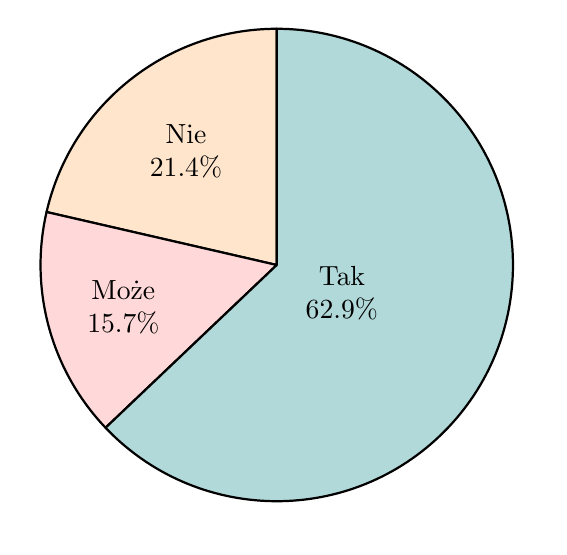
\begin{tikzpicture}
\pie[text = inside, rotate=90, color ={orange!20, pink!60, teal!30}]
    {21.4/Nie, 15.7/Może, 62.9/Tak}
\end{tikzpicture}
\label{Wykres:2}
\caption{Czy zna Pan/Pani członków subkultury metalowej? -- odpowiedzi}
\end{figure}

Z pyt. 4 wynika, że respondenci mają wspólną wizję wyglądu zewnętrznego uczestnika subkultury metalowej. Czterdziestu siedmiu ankietowanych podaje ciemne ubrania i kolor czarny jako fundamentalną cechę wyglądu metalowca [patrz: Tabela \ref{table:2}]. Uwagę respondentów zdaje się także przyciągać charakterystyczne, wysokie obuwie metalowców. Zaprojektowane jako buty robocze glany, jedynie w obrębie subkultury funkcjonują jako obuwie codzienne. W połączeniu z czarnym strojem, stanowią bazę stylu heavymetalowego.


\begin{table}[!htb]
\begin{tabular}{ m{23em} | m{5em} } 
\textbf{Co jest charakterystyczne dla wyglądu zewnętrznego metalowca?} & Liczba odpowiedzi \\
\hline
czarne ubrania & 47 \\
glany & 41 \\
długie włosy & 38 \\
skórzane ubrania & 16 \\
ćwieki & 13 \\
piercing & 8 \\
tatuaże & 8 \\
łańcuchy & 8 \\
koszulki z nazwami zespołów metalowych & 7 \\
naszywki & 7 \\
pieszczocha & 6 \\
mocny makijaż & 5 \\
jeans & 4 \\
plecak kostka & 4 \\
zarost & 2 \\
\end{tabular} 
\caption{Co jest charakterystyczne dla wyglądu zewnętrznego metalowca? -- najczęstsze odpowiedzi}
\label{table:2}
\end{table}

Większość udzielanych odpowiedzi stanowią reprezentatywne elementy ubioru uczestników subkultury metalowej. Respondenci zdecydowanie rzadziej odnoszą się do charakterystycznych cech sylwetki i urody metalowców. Spośród nich wymieniają jedynie długie włosy (38 odpowiedzi), piercing i tatuaże, które niekoniecznie uznaje się za typowe dla członków subkultury metalowej, oraz mocny makijaż i (wymieniony zaledwie 2 razy) zarost. Być może wynika to z tego, że zdaniem respondentów, to, co odróżnia metalowca wizualnie od przeciętnego człowieka, to przede wszystkim jego strój. 

Wydaje się, że w swoim opisie, ankietowani uwzględniali głównie metalowców płci męskiej, o czym świadczyć mogą długie włosy jako jedna z najczęściej wskazywanych cech dystynktywnych metalowców. U mężczyzn długie włosy wciąż mogą być uznawane za osobliwe -- stoją w niezgodzie z przyjętą w Polsce konwencją, a w społecznościach katolickich jawią się jako przejaw buntu i "niechęci do schematów".\footnote{http://adonai.pl/relaks/psychologia/?id=10} Według psychologicznego portalu katolickiego Adonai, ta sama fryzura u kobiet świadczy z kolei o "świadomej kobiecości"\footnote{Tamże.} i mieści się w ramach obowiązujących społecznych norm. 

Tylko cztery razy pada odpowiedź, że metalowców charakteryzuje mocny makijaż, który potraktowany może zostać jako cecha reprezentatywna kobiet przynależących do analizowanej subkultury. Równie rzadko badani zwykli wspominać o plecakach tzw. kostkach oraz ubraniach wykonanych z jeansu, który stał się popularny we wszystkich środowiskach.

Część ankietowanych kładła nacisk na elementy ozdobne ubioru metalowców. Wśród nich najczęściej pojawiały się ćwieki (13 odpowiedzi) oraz metalowe łańcuchy. Nieco mniejszą popularnością wśród badanych cieszyły się pieszczochy oraz naszywki z logotypami zespołów metalowych [patrz: Tabela \ref{table:2}].

Zdaniem respondentów, metalowcy w życiu zawodowym wybierają różne ścieżki. 26 na 90 udzielonych na pyt. 5 odpowiedzi, zakłada, że metalowiec może podjąć się dowolnego zawodu [patrz: Tabela \ref{table:3}]. Trudne byłoby zatem jednoznaczne zdeterminowanie wyobrażenia większości respondentów na temat statusu majątkowego i/lub społecznego uczestnika subkultury metalowej. 

Niemniej jednak, wielu z ankietowanych kojarzy metalowców z twórcami muzyki metalowej, w drugiej kolejności zaś z osobami pracującymi w branży informatycznej [patrz: Tabela \ref{table:3}], które można uznać za najlepiej płatne spośród wszystkich wymienianych przez respondentów stanowisk pracy. Wśród wymienianych profesji, przeważają jednak te średniodochodowe, a 6 osób stwierdza, że metalowcy to jeszcze ludzie młodzi, nie podejmujący pracy zarobkowej. Czterech ankietowanych uważa, że metalowcy to osoby o niskim statusie społecznym, posiadające status bezrobotnych.  


\begin{table}[!tp]
\begin{tabular}{ m{23em} | m{5em} } 
\textbf{Jaki zawód wykonuje metalowiec?} & Liczba odpowiedzi \\
\hline
każdy & 26 \\
muzyk & 18 \\
programista/informatyk & 8 \\
sprzedawca & 6 \\
uczy się & 6 \\
nie wiem & 5 \\
mechanik & 5 \\
bezrobotny & 4 \\
barman & 3 \\
robotnik & 3 \\
tatuator & 2 \\
tester gier & 2 \\
kierowca & 2 \\
\end{tabular} 
\caption{Jaki wykonuje zawód? -- najczęstsze odpowiedzi}
\label{table:3}
\end{table}
%gwalcenie tabel i figur: [!htb]
\newpage
\begin{table}[!htb]
\begin{tabular}{ m{23em} | m{5em} } 
\textbf{Co metalowiec robi w wolnym czasie?
} & Liczba odpowiedzi \\
\hline
słucha muzyki & 31 \\
chodzi na koncerty & 26 \\
gra na instrumentach & 19 \\
to, co wszyscy & 12 \\
spotyka się ze znajomymi & 9 \\
imprezuje & 6 \\
spotyka się z innymi metalowcami & 3 \\
jeździ na motocyklu & 3 \\
ogląda filmy & 3 \\
nie wiem & 3 \\
czyta książki & 1 \\
zażywa narkotyki & 1 \\
\end{tabular} 
\caption{Co metalowiec robi w wolnym czasie? -- najczęstsze odpowiedzi}
\label{table:4}
\end{table}

W rozumieniu respondentów, metalowcy wolny czas spędzają słuchając muzyki oraz uczestnicząc w koncertach [patrz: Tabela \ref{table:4}]. Jak wynikało także z poprzedniego pytania, wielu z nich kojarzy metalowców nie tylko z biernymi słuchaczami muzyki metalowej, ale także z jej twórcami. Dziewiętnastu ankietowanych uważa, że w czasie wolnym, metalowcy oddają się pasji grania na instrumentach i tworzenia muzyki [patrz: Tabela \ref{table:4}] -- aż czternastu z nich sądzi, że metalowcy doskonalą umiejętność gry na gitarze. Jednakże na pyt. 1, tylko 8 osób odpowiedziało, że metalowcy są muzykalni, a jeszcze mniej, że cechują się kreatywnością [patrz: Tabela \ref{table:1}].



Na 70 przebadanych osób, jedna uważa, że fani metalu w czasie wolnym zażywają substancje psychoaktywne. 6 z nich kojarzy metalowców z imprezami, zwykle o charakterze domówki bądź imprezy plenerowej. Choć w wyobrażeniu sporej części grupy kontrolnej, metalowcy są zamkniętymi w sobie introwertykami [patrz: Tabela \ref{table:1}], 11 osób wierzy, że spędzają oni czas ze znajomymi -- w tym 3 osoby, które konkretnie wskazują innych metalowców jako ich bliskich [patrz: Tabela \ref{table:4}].

17 proc. respondentów uważa z kolei, że przynależący do subkultury osobnicy, posiadają zróżnicowane zainteresowania i w wolnym czasie oddają się takim samym czynnościom, jak ci, którzy do niej nie należą. W ich rozumieniu, metalowcy są osobami z różnymi pasjami, które nie są wypadkową ich uczestnictwa w subkulturze metalowej.

\chapter*{Zakończenie}
\addcontentsline{toc}{chapter}{Zakończenie}
\chapter*{Bibliografia}
\addcontentsline{toc}{chapter}{Bibliografia}

\end{document}
